\section{ANÁLISE E MODELAGEM DO SISTEMA WeFIND}

A transição entre o diagnóstico empírico dos problemas enfrentados pela sociedade e a efetiva construção de uma ferramenta de software demanda rigor analítico e formalismo técnico. No ciclo de engenharia de software, essa transição materializa-se na fase de análise e modelagem de sistemas, etapa responsável por traduzir as carências e os anseios identificados junto aos tutores em especificações lógicas estruturadas, regras de negócio inequívocas e diagramas visuais padronizados (PRESSMAN; MAXIM, 2021; SOMMERVILLE, 2019).

Como elucida Valente (2023), uma modelagem criteriosa cumpre três objetivos capitais: estabelece a base conceitual compartilhada entre desenvolvedores e usuários finais, define com precisão as fronteiras e responsabilidades do sistema computacional e antecipa a descoberta de inconsistências ou omissões arquiteturais que, se postergadas para a etapa de codificação, gerariam impactos severos de custo, tempo e retrabalho.

No projeto WeFIND, o processo de análise apoiou-se na elicitação de 43 requisitos funcionais e 14 requisitos não funcionais, fundamentados nos achados da pesquisa de campo (Capítulo 3) e orientados pelas normas de qualidade de produto da família ISO/IEC 25010 (ISO, 2023). Complementarmente, a especificação comportamental e conceitual do sistema foi documentada por meio da \textit{Unified Modeling Language} (UML), utilizando-se diagramas de casos de uso para mapear as interações dos perfis de usuário e diagramas de classes de domínio para formalizar a estrutura estática das informações persistidas.

As seções a seguir detalham a engenharia de requisitos, a organização modular das funções do aplicativo e os modelos gráficos representativos do ecossistema WeFIND.

\clearpage

\subsection{Engenharia e Levantamento de Requisitos}

A engenharia de requisitos constitui a espinha dorsal de qualquer projeto de tecnologia, pois formaliza exatamente o que a aplicação deve realizar e sob quais restrições e qualidades operacionais deve funcionar (SOMMERVILLE, 2019). A elicitação de requisitos do WeFIND decorreu da triangulação metodológica descrita no Capítulo 3: as dores manifestadas pelos 20 tutores entrevistados no levantamento de campo evidenciaram a carência de um mapa interativo e de canais de comunicação privativos, enquanto a análise comparativa de plataformas similares revelou a ausência de recursos preventivos acessíveis e gratuitos.

Para estruturar o desenvolvimento de maneira modular e garantir a rastreabilidade direta entre cada funcionalidade e seu respectivo objetivo operacional, os 43 requisitos funcionais estabelecidos foram organizados em oito módulos sistêmicos integrados.

O módulo de gestão de contas, acesso e perfil (abrangendo os requisitos RF01 a RF08) concentra os fluxos de cadastro de usuário, autenticação persistente com sessão em nuvem, recuperação segura de credenciais por redefinição de senha via WhatsApp, consulta e atualização dos dados cadastrais e foto de perfil, encerramento protegido da sessão, painel central de notificações e o acesso público em modo visitante sem obrigatoriedade de login prévio. Em sequência, o módulo de publicações e gestão de ocorrências (RF09 a RF17) viabiliza o registro de animais nas categorias de perdidos, encontrados ou para adoção com upload fotográfico, seleção mandatória do ponto geográfico no mapa, indicação opcional de tutor terceiro, ordenação espacial dinâmica no feed de notícias, filtragem multicritério simultânea, exibição de detalhes completos da ocorrência, edição, encerramento com sucesso e exclusão definitiva de publicações.

A exploração cartográfica e navegação espacial (RF18 a RF21) organiza a renderização dos marcadores coloridos diferenciados por espécie sobre o mapa (abrangendo cães, gatos, aves e outros animais domésticos), disponibiliza mecanismos de busca e filtragem em tempo real sobre os pontos geográficos, permite o ajuste contínuo do raio de busca de proximidade e realiza o cálculo automatizado de rotas viárias com estimativa de tempo e distância até o animal. Complementarmente, o módulo de rastreamento colaborativo e avistamentos (RF22 a RF27) assegura o registro comunitário de avistamentos de animais soltos com coordenadas e fotografia pelo informante, organizando uma linha do tempo cronológica na publicação, além de possibilitar a manutenção de relatos pelo autor e a atualização dinâmica do marcador principal do pet no mapa conforme novos relatos confirmados.

A prevenção e a guarda responsável consolidam-se no módulo de Cadastro de Animais Tutelados (RF28 a RF33), possibilitando o registro preventivo dos animais domésticos sob responsabilidade do tutor contendo histórico veterinário e vacinal, a geração da ficha de identificação com código QR exclusivo para acoplamento em coleiras, a manutenção cadastral contínua e o acionamento de alerta de desaparecimento em caso de fuga imprevista. Para ampliar a visibilidade dos casos, o módulo de suporte à divulgação externa e cartazes digitais (RF34 a RF36) fornece a geração automatizada de peças gráficas diagramadas com fotografia, dados vitais e código QR inteligente, oferecendo suporte aos formatos padronizados para impressão física em folha A4 e publicação em Stories e Feed de redes sociais, integrado ao painel de compartilhamento nativo do smartphone.

Por fim, a comunicação direta e a integridade da comunidade são asseguradas por dois módulos essenciais. O módulo de canal privativo de comunicação e chat (RF37 a RF39) estrutura o diálogo direto e em tempo real entre quem perdeu e quem encontrou o pet, viabilizando a troca instantânea de mensagens de texto via WebSockets e o envio de fotografias comprobatórias de identidade física do animal, eliminando a exposição de telefones particulares em vias públicas. Simultaneamente, o módulo de governança comunitária, reencontros e moderação (RF40 a RF43) promove o engajamento comunitário por meio da publicação e consulta de histórias felizes de reencontro no mural colaborativo, garantindo a integridade da plataforma através de denúncias comunitárias de anúncios impróprios e rotinas administrativas de auditoria, moderação e suspensão de contas fraudulentas.

\clearpage

\subsubsection{Requisitos Funcionais}

O Quadro~\ref{quadro:funcionais} consolida a especificação integral dos 43 requisitos funcionais do aplicativo WeFIND, indicando para cada item o respectivo identificador unívoco, a denominação operacional e a descrição do comportamento esperado pelo sistema.

\vspace{0.3cm}
{
\phantomsection\label{quadro:funcionais}
\small
\renewcommand{\arraystretch}{1.18}
\begin{longtable}{|>{\centering\arraybackslash}p{1.3cm}|>{\raggedright\arraybackslash}p{4.2cm}|>{\raggedright\arraybackslash}p{8.8cm}|}
\hline
\multicolumn{3}{|c|}{\textbf{Quadro 2: Requisitos Funcionais do Sistema WeFIND}} \\ \hline
\textbf{ID} & \textbf{Nome do Requisito} & \textbf{Descrição do Comportamento Esperado} \\ \hline
\endfirsthead

\hline
\multicolumn{3}{|c|}{\textbf{Quadro 2: Requisitos Funcionais do Sistema WeFIND (Continuação)}} \\ \hline
\textbf{ID} & \textbf{Nome do Requisito} & \textbf{Descrição do Comportamento Esperado} \\ \hline
\endhead

\hline
\multicolumn{3}{|r|}{\textit{Continua na próxima página}} \\ \hline
\endfoot

\hline
\multicolumn{3}{|l|}{\textbf{Fonte:} Autoria própria (2026)} \\ \hline
\endlastfoot

\textbf{RF01} & Cadastrar Usuário & Permitir a criação de conta fornecendo nome completo, e-mail, telefone e senha de acesso. \\ \hline
\textbf{RF02} & Autenticar Usuário (Login) & Validar credenciais de acesso e iniciar sessão persistente no aplicativo via Supabase Auth. \\ \hline
\textbf{RF03} & Redefinir Senha de Acesso & Permitir a recuperação de conta esquecida por meio de envio de código seguro via WhatsApp. \\ \hline
\textbf{RF04} & Consultar Perfil de Usuário & Exibir informações de cadastro, foto de perfil, dados de contato e histórico de atividades do usuário. \\ \hline
\textbf{RF05} & Editar Dados de Perfil & Permitir a atualização de nome, foto, WhatsApp com confirmação em duas etapas, redes sociais e localização GPS com raio de busca. \\ \hline
\textbf{RF06} & Encerrar Sessão (Logout) & Finalizar a sessão ativa no dispositivo móvel de forma segura, limpando dados temporários e credenciais em cache. \\ \hline
\textbf{RF07} & Consultar Notificações & Apresentar painel com avisos sobre novos avistamentos, mensagens recebidas e alertas de publicações próximas. \\ \hline
\textbf{RF08} & Permitir Modo Visitante & Disponibilizar acesso público inicial para consulta de publicações e navegação no mapa sem exigir login imediato. \\ \hline
\textbf{RF09} & Cadastrar Publicação & Registrar nova publicação de animal (Perdido, Encontrado ou Adoção) com fotos, atributos físicos e descrição. \\ \hline
\textbf{RF10} & Selecionar Localização da Publicação & Abrir mapa interativo para o usuário fixar as coordenadas geográficas exatas onde o fato ocorreu. \\ \hline
\textbf{RF11} & Informar Tutor Terceiro & Permitir ao usuário que encontrou um animal cadastrar dados de contato de uma terceira pessoa responsável pela guarda. \\ \hline
\textbf{RF12} & Listar Publicações no Feed & Exibir anúncios ativos ordenados dinamicamente por menor distância física em relação ao usuário e data de publicação. \\ \hline
\textbf{RF13} & Filtrar e Buscar Publicações & Permitir filtragem simultânea por espécie, status (Perdido/Encontrado/Adoção), porte, sexo e raio de distância. \\ \hline
\textbf{RF14} & Consultar Detalhes da Publicação & Apresentar tela completa da publicação com fotos ampliadas, características físicas e botão de contato com o autor. \\ \hline
\textbf{RF15} & Editar Dados da Publicação & Permitir ao autor do anúncio atualizar fotos, características físicas, descrições e telefones de contato informados. \\ \hline
\textbf{RF16} & Atualizar Status da Publicação & Permitir ao autor alterar o status da publicação para ``Reencontrado'' ou ``Adotado'', encerrando as buscas ativas. \\ \hline
\textbf{RF17} & Excluir Publicação & Permitir ao autor remover permanentemente o anúncio cadastrado da base de dados e do mapa. \\ \hline
\textbf{RF18} & Visualizar Animais no Mapa & Apresentar mapa interativo com marcadores coloridos identificando animais perdidos, encontrados e disponíveis para adoção. \\ \hline
\textbf{RF19} & Pesquisar Marcadores no Mapa & Filtrar em tempo real os marcadores exibidos no mapa de acordo com termos de busca e atributos do pet. \\ \hline
\textbf{RF20} & Ajustar Raio de Proximidade & Permitir configurar a distância de abrangência da busca geográfica no mapa (de 5 km até todo o território nacional). \\ \hline
\textbf{RF21} & Traçar Rota GPS até o Ponto & Calcular e desenhar no mapa o trajeto viário e estimativa de deslocamento até o local onde o animal foi visto. \\ \hline
\textbf{RF22} & Cadastrar Avistamento & Permitir a qualquer usuário relatar que avistou um pet perdido, anexando nova foto, coordenadas e descrição do local. \\ \hline
\textbf{RF23} & Selecionar Local do Avistamento & Abrir o mapa interativo para posicionar o marcador no local exato onde o animal foi avistado em via pública. \\ \hline
\textbf{RF24} & Listar Histórico de Avistamentos & Exibir linha do tempo na publicação com todos os relatos de avistamentos registrados pela comunidade. \\ \hline
\textbf{RF25} & Editar Dados do Avistamento & Permitir ao autor do avistamento atualizar detalhes, fotos ou referências do relato cadastrado. \\ \hline
\textbf{RF26} & Excluir Registro de Avistamento & Permitir a remoção de um relato de avistamento incorreto ou duplicado da linha do tempo da publicação. \\ \hline
\textbf{RF27} & Atualizar Posição por Avistamento & Atualizar a posição do marcador principal do pet no mapa para o ponto do avistamento confirmado mais recente. \\ \hline
\textbf{RF28} & Cadastrar Pet Preventivo (Meu Pet) & Registrar preventivamente os animais domésticos da família com nome, espécie, raça, vacinas e contatos do tutor. \\ \hline
\textbf{RF29} & Listar Pets Cadastrados & Apresentar painel com todos os animais domésticos tutelados pelo usuário cadastrados preventivamente. \\ \hline
\textbf{RF30} & Consultar Identificação do Animal Tutelado & Apresentar a ficha cadastral de identificação do animal contendo foto, dados do tutor e código QR exclusivo. \\ \hline
\textbf{RF31} & Editar Dados de Meu Pet & Permitir ao tutor atualizar fotos, registros veterinários, vacinas e características físicas dos animais tutelados. \\ \hline
\textbf{RF32} & Excluir Cadastro de Meu Pet & Permitir ao tutor excluir definitivamente o registro preventivo de um animal do seu perfil. \\ \hline
\textbf{RF33} & Acionar Alerta de Desaparecimento & Converter instantaneamente o cadastro do animal tutelado em publicação de busca no mapa sem redigitar dados. \\ \hline
\textbf{RF34} & Gerar Cartaz de Busca & Criar automaticamente cartaz de divulgação contendo fotografia, dados essenciais da publicação e código QR escaneável. \\ \hline
\textbf{RF35} & Escolher Formato do Cartaz & Permitir a geração da peça gráfica em múltiplos formatos (A4 para impressão em postes, 9:16 para Stories e 1:1 para Feed). \\ \hline
\textbf{RF36} & Compartilhar Cartaz Digital & Integrar com o compartilhamento nativo do sistema operacional para envio direto da imagem em redes e mensageiros. \\ \hline
\textbf{RF37} & Iniciar Conversa via Chat & Abrir canal de diálogo direto e privativo entre o interessado e o autor de uma publicação específica. \\ \hline
\textbf{RF38} & Trocar Mensagens em Tempo Real & Viabilizar o envio e recebimento instantâneo de mensagens de texto entre usuários conectados via WebSockets. \\ \hline
\textbf{RF39} & Enviar Imagens no Chat & Permitir o envio de fotos na conversa privativa para conferência de características físicas e identificação segura do animal. \\ \hline
\textbf{RF40} & Cadastrar História Feliz & Permitir ao tutor cujo pet foi localizado publicar um relato de agradecimento com fotos no mural comunitário. \\ \hline
\textbf{RF41} & Listar Histórias Felizes no Mural & Exibir mural público comunitário com relatos e fotos de animais que foram resgatados ou reencontrados com sucesso. \\ \hline
\textbf{RF42} & Denunciar Publicação Suspeita & Permitir que os usuários reportem anúncios falsos, suspeitos ou com conteúdo impróprio à equipe de moderação. \\ \hline
\textbf{RF43} & Gerenciar Denúncias e Moderação & Permitir ao administrador listar denúncias, analisar publicações reportadas, remover conteúdos impróprios e suspender contas. \\ \hline
\end{longtable}
}

\clearpage

\subsubsection{Requisitos Não Funcionais}

Enquanto os requisitos funcionais estabelecem as ações e serviços oferecidos pela aplicação móvel, os requisitos não funcionais especificam as restrições arquiteturais, os critérios de qualidade do produto e os padrões de desempenho sob os quais o sistema deve operar (VALENTE, 2023). A definição desses parâmetros fundamentou-se na norma internacional ISO/IEC 25010 (ISO, 2023), englobando aspectos de eficiência de desempenho, compatibilidade multiplataforma, segurança da informação e confiabilidade.

O Quadro~\ref{quadro:nao_funcionais} sintetiza os 14 requisitos não funcionais estabelecidos para a plataforma WeFIND, organizados por critérios mensuráveis de aceitação.

\vspace{0.3cm}
{
\phantomsection\label{quadro:nao_funcionais}
\small
\renewcommand{\arraystretch}{1.18}
\begin{longtable}{|>{\centering\arraybackslash}p{1.4cm}|>{\raggedright\arraybackslash}p{3.8cm}|>{\raggedright\arraybackslash}p{9.2cm}|}
\hline
\multicolumn{3}{|c|}{\textbf{Quadro 3: Requisitos Não Funcionais do Sistema WeFIND}} \\ \hline
\textbf{ID} & \textbf{Critério de Qualidade} & \textbf{Métrica Mensurável / Restrição Arquitetural} \\ \hline
\endfirsthead

\hline
\multicolumn{3}{|c|}{\textbf{Quadro 3: Requisitos Não Funcionais do Sistema WeFIND (Continuação)}} \\ \hline
\textbf{ID} & \textbf{Critério de Qualidade} & \textbf{Métrica Mensurável / Restrição Arquitetural} \\ \hline
\endhead

\hline
\multicolumn{3}{|r|}{\textit{Continua na próxima página}} \\ \hline
\endfoot

\hline
\multicolumn{3}{|l|}{\textbf{Fonte:} Autoria própria (2026)} \\ \hline
\endlastfoot

\textbf{RNF01} & Desempenho de Inicialização & O aplicativo deve carregar sua interface inicial e exibir os anúncios em tempo inferior a 2,0 segundos sob conexões de rede 4G. \\ \hline
\textbf{RNF02} & Latência de Mensagens no Chat & A transmissão e exibição de mensagens de texto entre usuários no chat em tempo real deve ocorrer em menos de 500 ms via WebSockets. \\ \hline
\textbf{RNF03} & Compressão Local de Imagens & Todas as fotografias selecionadas para anúncios devem passar por compressão algorítmica no próprio aparelho, limitando o arquivo a no máximo 500 KB antes do upload. \\ \hline
\textbf{RNF04} & Precisão de Geolocalização & A captura de localização do dispositivo móvel via GPS nativo deve operar com margem de precisão horizontal inferior a 15 metros. \\ \hline
\textbf{RNF05} & Proteção de Dados e Anonimização & O sistema não deve exibir em mapa público o endereço residencial exato do usuário, aplicando máscara de aproximação territorial por bairro. \\ \hline
\textbf{RNF06} & Anonimato de Lares Temporários & A localização física de voluntários cadastrados para acolhimento de lar temporário deve ser estritamente preservada, mantendo oculto o endereço exato. \\ \hline
\textbf{RNF07} & Segurança de Autenticação & A infraestrutura de autenticação do Supabase Auth deve armazenar credenciais com hash criptográfico seguro (bcrypt) e emitir tokens JWT válidos. \\ \hline
\textbf{RNF08} & Isolamento de Dados via RLS & As operações no banco de dados PostgreSQL devem impor políticas de segurança em nível de linha (RLS), impedindo acessos ou exclusões indevidas entre contas. \\ \hline
\textbf{RNF09} & Criptografia em Trânsito & Todo o tráfego de dados entre o aplicativo cliente móvel e a infraestrutura em nuvem deve ser obrigatoriamente cifrado via protocolo HTTPS e TLS 1.3. \\ \hline
\textbf{RNF10} & Acessibilidade e Contraste & As telas devem oferecer suporte a Modo Claro e Modo Escuro com contraste visual mínimo de 4.5:1 para conformidade com a norma WCAG nível AA. \\ \hline
\textbf{RNF11} & Compatibilidade Móvel & O aplicativo deve ser compilado e executado nativamente em dispositivos móveis Android (versão 7.0 ou superior) e iOS (versão 13 ou superior) via React Native. \\ \hline
\textbf{RNF12} & Design Responsivo de Telas & A interface deve adaptar-se dinamicamente a diferentes resoluções e densidades de pixels de smartphones, sem corte de texto ou sobreposição de botões. \\ \hline
\textbf{RNF13} & Disponibilidade da Nuvem & O backend em nuvem provido pelo Supabase deve assegurar taxa de disponibilidade de serviço mínima de 99,5\% com rotinas automatizadas de backup diário. \\ \hline
\textbf{RNF14} & Janela Ética de Adoção & O sistema deve aplicar regra de negócio bloqueando a alteração de status de um animal encontrado para adoção definitiva antes de decorridos 7 dias de busca ativa. \\ \hline
\end{longtable}
}

Em termos de engenharia, os requisitos não funcionais dividem-se em quatro pilares fundamentais. No primeiro pilar (eficiência e desempenho), o sistema assegura tempos de resposta céleres para carregamento inicial (RNF01) e propagação instantânea de mensagens (RNF02), associando mecanismos de compressão fotográfica prévia no dispositivo (RNF03) e calibração de GPS (RNF04).

No segundo pilar (segurança, criptografia e conformidade com a LGPD), o aplicativo assegura a supressão de endereços residenciais exatos nos mapas públicos (RNF05), proteção de localização para lares temporários de acolhimento (RNF06), autenticação segura de contas (RNF07), isolamento estrito de permissões no PostgreSQL por políticas de segurança em nível de linha (RNF08) e criptografia de ponta a ponta nas comunicações de rede via HTTPS e TLS (RNF09).

No terceiro pilar (usabilidade, acessibilidade e portabilidade), a aplicação oferece alternância entre modo claro e modo escuro com contraste estrito para uso sob luz solar direta (RNF10), compatibilidade multiplataforma entre sistemas operacionais Android e iOS via React Native (RNF11) e design responsivo com adaptação dinâmica a telas de diversas resoluções (RNF12).

Por fim, no quarto pilar (confiabilidade e regras éticas de negócio), a infraestrutura em nuvem assegura disponibilidade contínua mínima de 99,5\% com rotinas automatizadas de backup (RNF13) e impõe a janela de segurança de busca mínima de 7 dias antes de permitir a alteração de status de um animal resgatado para adoção definitiva (RNF14).

\clearpage

\subsection{Modelagem Conceitual e Estrutural do Sistema}

A modelagem de software é uma etapa fundamental no desenvolvimento de qualquer sistema, pois organiza visualmente a lógica, as regras e o funcionamento da aplicação antes e durante a escrita do código. Ao criar esquemas visuais padronizados, a equipe alinha as expectativas com os requisitos e evita inconsistências que poderiam comprometer a arquitetura ou a experiência de uso (BEZERRA, 2021).

No desenvolvimento da aplicação proposta, utilizou-se a \textit{Unified Modeling Language} (UML) como padrão para documentar o sistema. A UML permite enxergar o aplicativo por duas perspectivas complementares: a comportamental, expressa nos diagramas de casos de uso que apresentam as ações disponibilizadas a cada perfil de usuário; e a estrutural, representada pelo diagrama de classes de domínio.

\clearpage

\subsubsection{Diagrama de Casos de Uso}

O diagrama de casos de uso da \textit{Unified Modeling Language} (UML) estabelece a modelagem comportamental externa do sistema sob a ótica dos atores participantes, delimitando os objetivos operacionais, as fronteiras da aplicação e as interações disponibilizadas aos usuários e serviços parceiros (BEZERRA, 2021; VALENTE, 2023). Como enfatizam Pressman e Maxim (2021), a especificação de casos de uso não visa reproduzir exaustivamente cada rotina interna de validação ou instrução de banco de dados, mas sim consolidar os cenários de utilização que entregam valor direto aos usuários da solução tecnológica.

Diferente de abordagens fragmentadas que dividem os fluxos de forma desarticulada, optou-se pela concepção de um diagrama de casos de uso geral unificado. Esse modelo sintetiza, em uma única visão integrada e formalizada na ferramenta Astah UML, todas as permissões públicas de visitantes, os fluxos protegidos de usuários cadastrados, as rotinas de moderação administrativa e a comunicação com serviços externos. A Figura~\ref{fig:diagrama_casos_de_uso} ilustra o diagrama de casos de uso geral da plataforma WeFIND.

\begin{figure}[H]
    \centering
    \caption{Diagrama de Casos de Uso Geral da Plataforma WeFIND}
    \label{fig:diagrama_casos_de_uso}
    \vspace{0.2cm}
    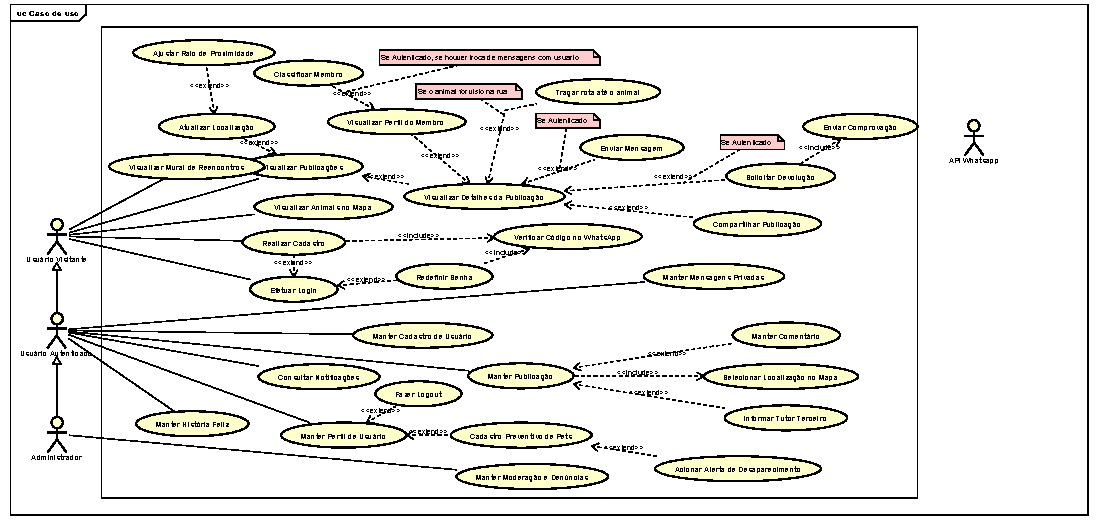
\includegraphics[width=\textwidth]{imagens/02_modelagem/figura06_diagrama_casos_de_uso.pdf}
    \vspace{0.1cm}
    \fonte{Autoria própria (2026)}
\end{figure}

A análise da arquitetura funcional apresentada na Figura~\ref{fig:diagrama_casos_de_uso} evidencia uma estrutura rigorosamente orientada aos objetivos operacionais do sistema, organizada em torno de quatro atores e módulos funcionais interdependentes:

\paragraph{Atores do Sistema e Regra de Generalização:} O ecossistema define três atores humanos primários e um ator secundário tecnológico:
\begin{enumerate}[label=\alph*)]
    \item \textbf{Usuário Visitante:} ator primário que acessa o aplicativo sem necessidade de autenticação prévia. Dispõe de acesso irrestrito às ações de utilidade pública: consultar publicações de animais no feed contínuo, explorar marcadores georreferenciados no mapa interativo, consultar o mural comunitário de reencontros felizes, acessar os detalhes completos de qualquer publicação, realizar cadastro de nova conta ou efetuar login na plataforma.
    \item \textbf{Usuário Autenticado:} cidadão ou tutor com conta validada por verificação de telefone celular. No diagrama, modelou-se uma relação formal de \textbf{generalização/herança} da UML entre os atores, indicada pela seta com triângulo vazado direcionada ao \textit{Usuário Visitante} (\textit{Usuário Autenticado} herda de \textit{Usuário Visitante}). Esse relacionamento estabelece que o usuário autenticado herda nativamente todas as funções públicas do visitante, agregando adicionalmente as permissões de escrita, comunicação segura, publicação georreferenciada e salvaguarda preventiva de animais tutelados.
    \item \textbf{Administrador:} ator responsável pela governança ética e segurança da plataforma, atuando no caso de uso especializado de moderação e auditoria de denúncias.
    \item \textbf{API WhatsApp:} ator tecnológico secundário (sistema externo), acionado de forma programática pelo backend para entrega de códigos numéricos de autenticação temporária (OTP) e alertas imediatos.
\end{enumerate}

\paragraph{Módulo de Identidade, Autenticação e Acesso Seguro:} A entrada na plataforma estrutura-se pelos casos de uso \textit{Realizar Cadastro} e \textit{Efetuar Login}. A criação de conta estabelece uma dependência obrigatória de inclusão (\textit{«include»}) com o caso de uso \textit{Verificar Código no WhatsApp}, impedindo o registro de contas fraudulentas ou com números inexistentes. O caso de uso \textit{Efetuar Login} conecta-se à extensão opcional (\textit{«extend»}) \textit{Redefinir Senha}, permitindo ao usuário recuperar o acesso mediante revalidação por código via WhatsApp (\textit{«include» Verificar Código no WhatsApp}). Complementarmente, o gerenciamento de identidade é sustentado por \textit{Manter Cadastro de Usuário} e \textit{Manter Perfil de Usuário}, do qual deriva a extensão de saída segura \textit{Fazer Logout}.

\paragraph{Módulo de Descoberta Espacial e Consulta Cartográfica:} A visualização de animais apoia-se em \textit{Visualizar Publicações} (disposição vertical em feed contínuo ordenado por proximidade) e \textit{Visualizar Animais no Mapa} (renderização cartográfica com marcação colorida por status operacional). A exploração no mapa integra duas extensões: \textit{Ajustar Raio de Proximidade}, viabilizando a calibragem do filtro de busca entre bairros contíguos ou âmbito nacional, e \textit{Atualizar Localização}, que sincroniza a posição do usuário via satélite GPS.

\paragraph{Ações Especializadas a partir do Detalhe da Publicação:} A consulta aprofundada ao anúncio (\textit{Visualizar Detalhes da Publicação}) funciona como ponto central de convergência para decisões do usuário, disponibilizando cinco extensões condicionais (\textit{«extend»}):
\begin{itemize}
    \item \textit{Traçar rota até o animal}: estende a visualização mediante o ponto de extensão condicional \textit{``Se o animal for visto na rua''}, integrando a API de roteamento para desenhar trajetos viários e calcular tempos de deslocamento até o ponto onde o pet foi avistado;
    \item \textit{Enviar Mensagem}: recurso disponível sob a condição \textit{``Se Autenticado''}, conectando-se ao módulo \textit{Manter Mensagens Privadas} para conversação em tempo real sem expor números telefônicos particulares;
    \item \textit{Solicitar Devolução}: voltada à reivindicação de tutela sob a condição \textit{``Se Autenticado''}, incorporando como requisito mandatório (\textit{«include»}) o caso de uso \textit{Enviar Comprovação} (anexo de fotografias históricas, registros veterinários ou comprovantes de tutela);
    \item \textit{Compartilhar Publicação}: gera automaticamente cartazes digitais diagramados com código QR escaneável para difusão externa;
    \item \textit{Visualizar Perfil do Membro}: exibe o histórico comunitário do anunciante, admitindo a extensão \textit{Classificar Membro} sob a condição de guarda \textit{``Se Autenticado, se houver troca de mensagens com usuario''}, consolidando o mecanismo de reputação comunitária.
\end{itemize}

\paragraph{Módulo de Publicação, Comentários e Gestão Comunitária:} O anúncio de animais é formalizado no caso de uso \textit{Manter Publicação}, que executa as operações CRUD completas. Para assegurar integridade espacial, este caso inclui compulsoriamente (\textit{«include»}) \textit{Selecionar Localização no Mapa} para garantia de georreferenciamento exato, e admite as extensões opcionais \textit{Informar Tutor Terceiro} (quando o animal resgatado permanece com pessoa distinta do anunciante) e \textit{Manter Comentário} (destinado a relatos colaborativos de avistamento e pistas da vizinhança).

\paragraph{Módulo de Prevenção e Alerta Imediato:} A guarda responsável e a prevenção contra perdas definitivas articulam-se a partir de \textit{Manter Perfil de Usuário}, que se estende para \textit{Cadastro Preventivo de Pets}. Essa rotina viabiliza o registro antecipado de animais da família com dados clínicos, vacinas e carteirinha digital com código QR. Em caso de fuga imprevista, aciona-se a extensão \textit{Acionar Alerta de Desaparecimento}, que converte instantaneamente os dados do animal tutelado em publicação ativa de perda no mapa, alertando moradores próximos sem exigir a redigitação de fotos e atributos morfológicos.

\paragraph{Módulo de Governança e Apoio Comunitário:} A integridade da plataforma é resguardada por \textit{Manter Moderação e Denúncias}, acessível ao ator \textit{Administrador} para sanção de anúncios ilícitos e suspensão de contas fraudulentas. Em contrapartida, os reencontros bem-sucedidos são celebrados em \textit{Visualizar Mural de Reencontros} e \textit{Manter História Feliz}, enquanto o recebimento de alertas contínuos é estruturado em \textit{Consultar Notificações}.

\clearpage

\paragraph{Mapeamento de Rastreabilidade (Requisitos Funcionais vs. Casos de Uso):}
Para demonstrar a cobertura integral do projeto de software segundo os preceitos da Engenharia de Requisitos (PRESSMAN; MAXIM, 2021; SOMMERVILLE, 2019), o Quadro~\ref{quadro:mapeamento_rf_uc} formaliza a matriz de rastreabilidade bidirecional entre os 43 requisitos funcionais especificados no Quadro~\ref{quadro:funcionais} e os casos de uso modelados na Figura~\ref{fig:diagrama_casos_de_uso}, discriminando o ator responsável e a natureza do relacionamento UML.

\vspace{0.3cm}
{
\phantomsection\label{quadro:mapeamento_rf_uc}
\small
\setlength{\tabcolsep}{3.5pt}
\renewcommand{\arraystretch}{1.06}
\begin{longtable}{|>{\centering\arraybackslash}p{1.1cm}|>{\raggedright\arraybackslash}p{3.7cm}|>{\raggedright\arraybackslash}p{4.0cm}|>{\raggedright\arraybackslash}p{2.6cm}|>{\raggedright\arraybackslash}p{2.3cm}|}
\hline
\multicolumn{5}{|c|}{\textbf{Quadro 4: Mapeamento de Rastreabilidade entre Requisitos e Casos de Uso}} \\ \hline
\textbf{ID RF} & \textbf{Requisito Funcional} & \textbf{Caso de Uso Correspondente} & \textbf{Ator Primário} & \textbf{Relação UML} \\ \hline
\endfirsthead

\hline
\multicolumn{5}{|c|}{\textbf{Quadro 4: Mapeamento de Rastreabilidade entre Requisitos e Casos de Uso (Cont.)}} \\ \hline
\textbf{ID RF} & \textbf{Requisito Funcional} & \textbf{Caso de Uso Correspondente} & \textbf{Ator Primário} & \textbf{Relação UML} \\ \hline
\endhead

\hline
\multicolumn{5}{|r|}{\textit{Continua na próxima página}} \\ \hline
\endfoot

\hline
\multicolumn{5}{|l|}{\textbf{Fonte:} Autoria própria (2026)} \\ \hline
\endlastfoot

\textbf{RF01} & Cadastrar Usuário & Realizar Cadastro & Usuário Visitante & «include» (WhatsApp) \\ \hline
\textbf{RF02} & Autenticar Usuário (Login) & Efetuar Login & Usuário Visitante & Associação Direta \\ \hline
\textbf{RF03} & Redefinir Senha de Acesso & Redefinir Senha & Usuário Visitante & «extend» (Efetuar Login) \\ \hline
\textbf{RF04} & Consultar Perfil de Usuário & Manter Perfil de Usuário & Usuário Autenticado & Associação Direta \\ \hline
\textbf{RF05} & Editar Dados de Perfil & Manter Perfil de Usuário & Usuário Autenticado & Associação Direta \\ \hline
\textbf{RF06} & Encerrar Sessão (Logout) & Fazer Logout & Usuário Autenticado & «extend» (Manter Perfil) \\ \hline
\textbf{RF07} & Consultar Notificações & Consultar Notificações & Usuário Autenticado & Associação Direta \\ \hline
\textbf{RF08} & Permitir Modo Visitante & Acesso público aos casos de uso & Usuário Visitante & Associação Direta \\ \hline
\textbf{RF09} & Cadastrar Publicação & Manter Publicação & Usuário Autenticado & «include» (Localização) \\ \hline
\textbf{RF10} & Selecionar Localização da Publicação & Selecionar Localização no Mapa & Usuário Autenticado & «include» de Publicação \\ \hline
\textbf{RF11} & Informar Tutor Terceiro & Informar Tutor Terceiro & Usuário Autenticado & «extend» (Publicação) \\ \hline
\textbf{RF12} & Listar Publicações no Feed & Visualizar Publicações & Usuário Visitante & Associação Direta \\ \hline
\textbf{RF13} & Filtrar e Buscar Publicações & Visualizar Publicações & Usuário Visitante & Associação Direta \\ \hline
\textbf{RF14} & Consultar Detalhes da Publicação & Visualizar Detalhes da Publicação & Usuário Visitante & «extend» (Publicações) \\ \hline
\textbf{RF15} & Editar Dados da Publicação & Manter Publicação & Usuário Autenticado & Associação Direta \\ \hline
\textbf{RF16} & Atualizar Status da Publicação & Manter Publicação & Usuário Autenticado & Associação Direta \\ \hline
\textbf{RF17} & Excluir Publicação & Manter Publicação & Usuário Autenticado & Associação Direta \\ \hline
\textbf{RF18} & Visualizar Animais no Mapa & Visualizar Animais no Mapa & Usuário Visitante & Associação Direta \\ \hline
\textbf{RF19} & Pesquisar Marcadores no Mapa & Visualizar Animais no Mapa & Usuário Visitante & Associação Direta \\ \hline
\textbf{RF20} & Ajustar Raio de Proximidade & Ajustar Raio de Proximidade & Usuário Visitante & «extend» (Mapa) \\ \hline
\textbf{RF21} & Traçar Rota GPS até o Ponto & Traçar rota até o animal & Usuário Visitante & «extend» (Detalhes) \\ \hline
\textbf{RF22} & Cadastrar Avistamento & Manter Comentário & Usuário Autenticado & «extend» (Publicação) \\ \hline
\textbf{RF23} & Selecionar Local do Avistamento & Selecionar Localização no Mapa & Usuário Autenticado & «include» de Publicação \\ \hline
\textbf{RF24} & Listar Histórico de Avistamentos & Visualizar Detalhes da Publicação & Usuário Visitante & «extend» (Publicações) \\ \hline
\textbf{RF25} & Editar Dados do Avistamento & Manter Comentário & Usuário Autenticado & «extend» (Publicação) \\ \hline
\textbf{RF26} & Excluir Registro de Avistamento & Manter Comentário & Usuário Autenticado & «extend» (Publicação) \\ \hline
\textbf{RF27} & Atualizar Posição por Avistamento & Atualizar Localização & Usuário Visitante & «extend» (Mapa) \\ \hline
\textbf{RF28} & Cadastrar Pet Preventivo & Cadastro Preventivo de Pets & Usuário Autenticado & «extend» (Manter Perfil) \\ \hline
\textbf{RF29} & Listar Pets Cadastrados & Cadastro Preventivo de Pets & Usuário Autenticado & «extend» (Manter Perfil) \\ \hline
\textbf{RF30} & Consultar Identificação do Animal & Cadastro Preventivo de Pets & Usuário Autenticado & «extend» (Manter Perfil) \\ \hline
\textbf{RF31} & Editar Dados de Meu Pet & Cadastro Preventivo de Pets & Usuário Autenticado & «extend» (Manter Perfil) \\ \hline
\textbf{RF32} & Excluir Cadastro de Meu Pet & Cadastro Preventivo de Pets & Usuário Autenticado & «extend» (Manter Perfil) \\ \hline
\textbf{RF33} & Acionar Alerta de Desaparecimento & Acionar Alerta de Desaparecimento & Usuário Autenticado & «extend» (Cadastro Pet) \\ \hline
\textbf{RF34} & Gerar Cartaz de Busca & Compartilhar Publicação & Usuário Visitante & «extend» (Detalhes) \\ \hline
\textbf{RF35} & Escolher Formato do Cartaz & Compartilhar Publicação & Usuário Visitante & «extend» (Detalhes) \\ \hline
\textbf{RF36} & Compartilhar Cartaz Digital & Compartilhar Publicação & Usuário Visitante & «extend» (Detalhes) \\ \hline
\textbf{RF37} & Iniciar Conversa via Chat & Enviar Mensagem & Usuário Autenticado & «extend» (Detalhes) \\ \hline
\textbf{RF38} & Trocar Mensagens em Tempo Real & Manter Mensagens Privadas & Usuário Autenticado & Associação Direta \\ \hline
\textbf{RF39} & Enviar Imagens no Chat & Manter Mensagens Privadas & Usuário Autenticado & Associação Direta \\ \hline
\textbf{RF40} & Cadastrar História Feliz & Manter História Feliz & Usuário Autenticado & Associação Direta \\ \hline
\textbf{RF41} & Listar Histórias Felizes no Mural & Visualizar Mural de Reencontros & Usuário Visitante & Associação Direta \\ \hline
\textbf{RF42} & Denunciar Publicação Suspeita & Manter Moderação e Denúncias & Usuário Autenticado & Associação Direta \\ \hline
\textbf{RF43} & Gerenciar Denúncias e Moderação & Manter Moderação e Denúncias & Administrador & Associação Direta \\ \hline
\end{longtable}
}

\clearpage

\subsubsection{Diagrama de Classes de Domínio}

O diagrama de classes de domínio organiza as informações do sistema com base no paradigma orientado a objetos, formalizando as entidades essenciais do ecossistema WeFIND, seus atributos tipados com visibilidade, métodos de negócio e as relações estruturais da aplicação. A Figura~\ref{fig:diagrama_classes} apresenta o diagrama de classes de domínio da plataforma.

\begin{figure}[H]
    \centering
    \caption{Diagrama de Classes de Domínio do Sistema Proposto}
    \label{fig:diagrama_classes}
    \vspace{0.3cm}
    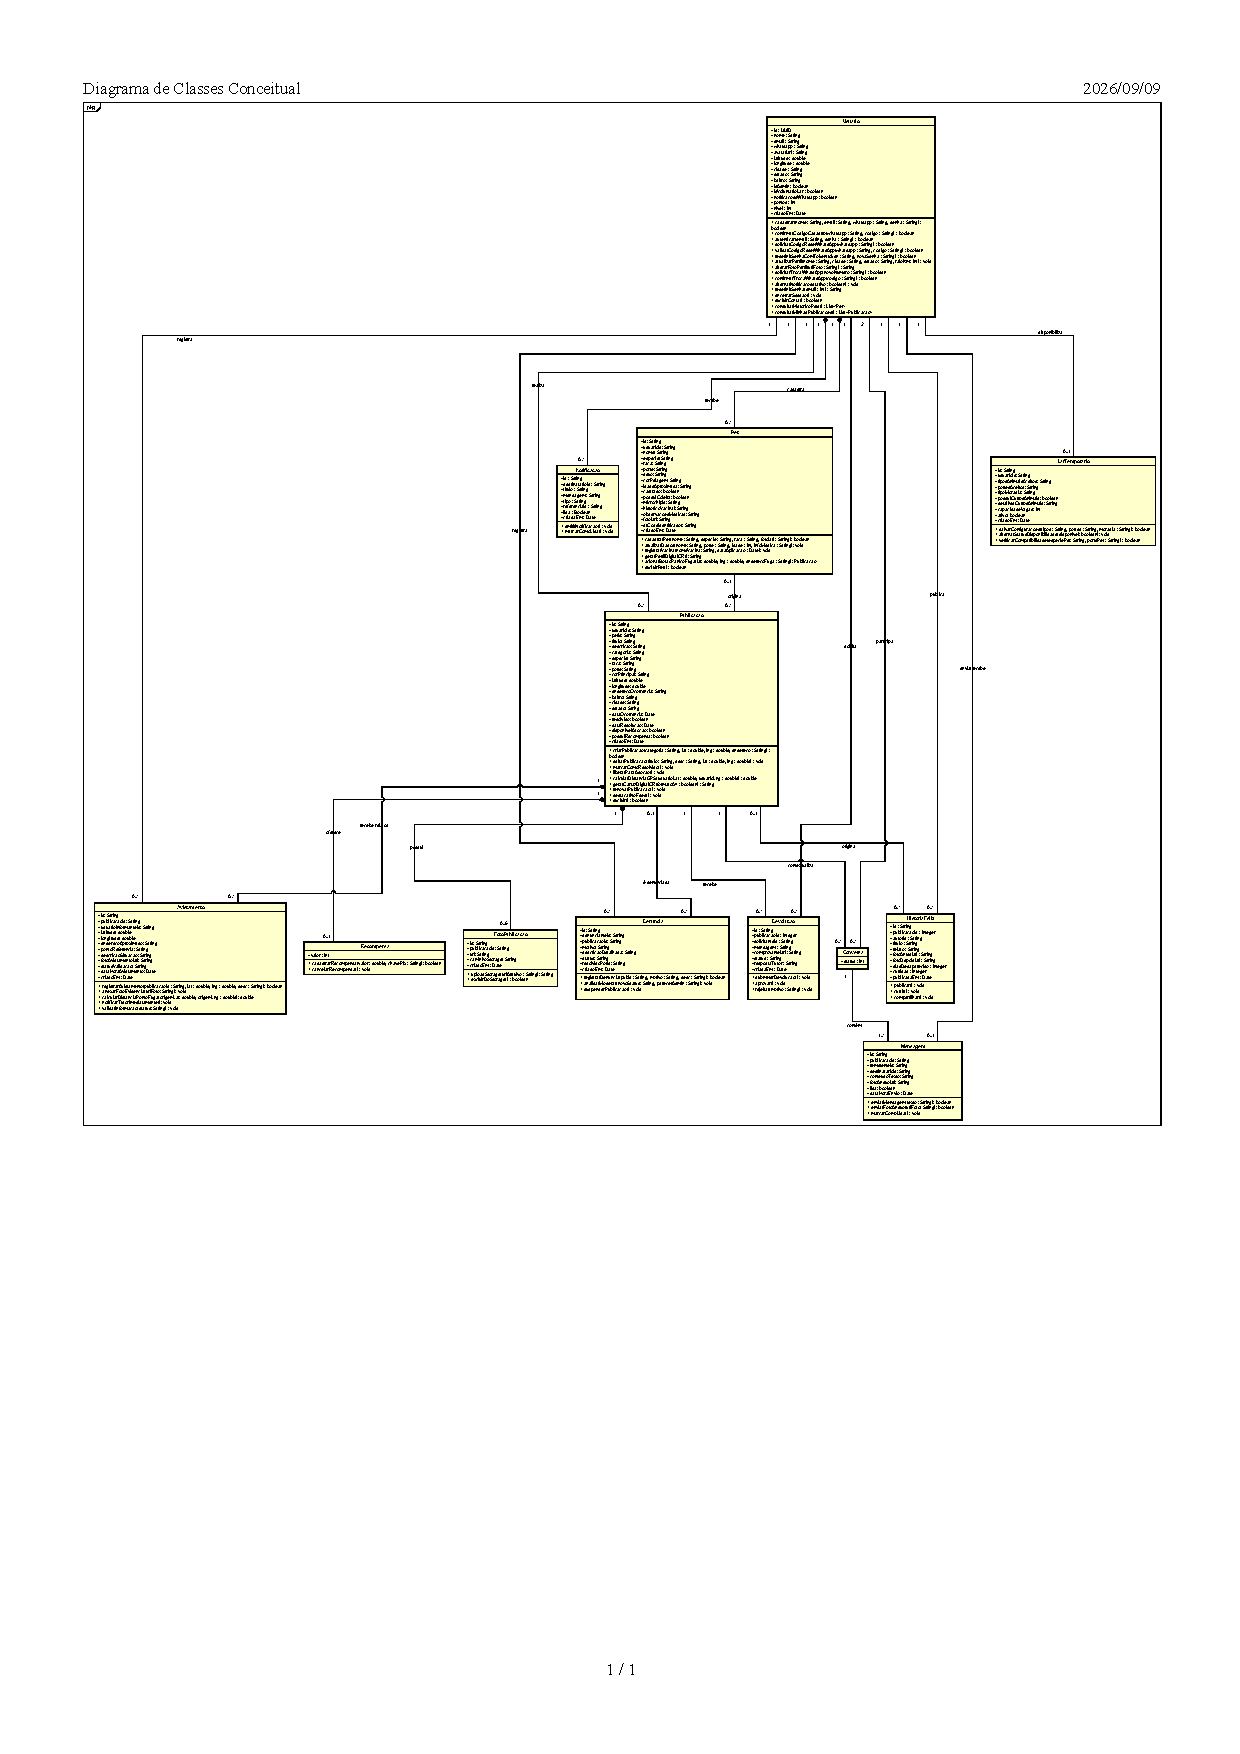
\includegraphics[trim=12mm 95mm 12mm 8mm, clip, width=0.99\textwidth]{imagens/02_modelagem/figura08_diagrama_classes.pdf}
    \vspace{0.1cm}
    \fonte{Autoria própria (2026)}
\end{figure}

\enlargethispage{2\baselineskip}
Na estrutura da Figura~\ref{fig:diagrama_classes}, os dados estão organizados a partir das classes centrais \textit{Usuario}, \textit{Pet} e \textit{Publicacao}, complementadas por módulos de apoio comunitário e governança. A classe \textit{Usuario} concentra a identidade do cidadão (identificador unívoco UUID, nome, e-mail, número de WhatsApp e foto de perfil) e suas referências espaciais (latitude, longitude, bairro, cidade, estado e raio de busca), além de gerenciar privilégios administrativos, engajamento por pontos e disponibilidade para lar temporário. Suas operações estruturam os fluxos de autenticação, redefinição de senha com validação de código e token via WhatsApp, atualização de localização no mapa e controle de notificações.

A classe \textit{Pet} viabiliza o cadastro preventivo de animais domésticos (abrangendo cães, gatos, aves, equinos e outros animais de companhia), registrando características físicas (raça, porte, sexo, pelagem e idade), cuidados veterinários (histórico vacinal e observações médicas), código de microchip eletrônico e identificador digital baseado em código QR. Destaca-se o método de acionamento de alerta de desaparecimento, que converte instantaneamente o cadastro do animal tutelado em uma nova ocorrência pública no sistema.

A classe \textit{Publicacao} representa os anúncios georreferenciados de animais perdidos, encontrados ou disponíveis para adoção. O registro armazena o ponto exato da ocorrência (latitude e longitude), endereço estruturado, dados morfológicos, datas de abertura e resolução, além de operações para cálculo de distância por GPS, renovação de expiração e geração automatizada de cartazes digitais diagramados. Cada anúncio pode incorporar de zero a seis imagens gerenciadas pela classe \textit{FotoPublicacao}, que provê métodos de integração com o armazenamento em nuvem (\textit{storage}).

A colaboração comunitária é viabilizada pela classe \textit{Avistamento}, que documenta coordenadas, fotos de evidência e a distância em relação ao ponto de fuga original. O acolhimento emergencial é estruturado pela classe \textit{LarTemporario}, que avalia a compatibilidade de espécies e portes frente à infraestrutura da moradia do voluntário. Por sua vez, a restituição formal de animais resgatados é mediada pela classe \textit{Devolucao}, com envio de comprovantes de tutela, podendo associar-se a uma bonificação gerenciada pela classe \textit{Recompensa} com chave PIX.

A comunicação segura entre os cidadãos ocorre por meio da classe \textit{Conversa}, que congrega instâncias da classe \textit{Mensagem} para tráfego instantâneo de texto e fotografias em tempo real via WebSockets. Por fim, a integridade da plataforma é assegurada pela classe \textit{Denuncia}, que permite reportar anúncios suspeitos para moderação administrativa, enquanto a classe \textit{HistoriaFeliz} fomenta a celebração de reencontros no mural comunitário e a classe \textit{Notificacao} distribui alertas geolocalizados aos usuários.

Com os requisitos funcionais formalizados e a modelagem de classes de domínio consolidada, o Capítulo 5 apresenta a plataforma WeFIND, detalhando sua proposta comunitária, a motivação do autor e a justificativa técnica para a abordagem móvel.

\clearpage
